\documentclass[12pt,letterpaper, onecolumn]{exam}
\usepackage{amsmath}
\usepackage{amssymb}
\usepackage{amsthm}
\usepackage{graphicx}
\usepackage{mathrsfs}
\usepackage{xcolor}
\usepackage[lmargin=71pt, tmargin=1.2in]{geometry}  %For centering solution box
\usepackage[english]{babel}
\newtheorem{theorem}{Theorem}
\newtheorem{lemma}[theorem]{Lemma}
\usepackage{accents}
\usepackage{ulem} % sout() to crossing things out 
\newcommand{\ubar}[1]{\underaccent{\bar}{#1}}
\newcommand{\bs}[1]{\boldsymbol{#1}}
\newcommand{\bm}[1]{\mathbf{#1}}
\newcommand{\der}[2]{\frac{d #1}{d#2}}
\newcommand{\pder}[3]{\frac{\delta^{#3} #1}{\delta^{#3}#2}}
\newcommand{\rs}{$X_1, ..., X_n$}
\newcommand{\nsum}{\sum_{i=1}^n}
\newcommand{\nprod}{\prod_{i=1}^n}
\newcommand*{\Comb}[2]{{}^{#1}C_{#2}}%
\newcommand{\ifc}{\textrm{ if }}
\newcommand{\real}{\mathbb{R}}
\newcommand{\nat}{\mathbb{N}}
\newcommand{\power}{\mathcal{P}}
\newcommand{\rational}{\mathbb{Q}}
\newcommand{\cutelim}{\lim\limits_{n\to\infty}}
\newcommand{\salg}{$\sigma$-algebra }

\newcommand{\calA}{\mathcal{A}}
\newcommand{\calO}{\mathcal{O}}
\newcommand{\calC}{\mathcal{C}}
\newcommand{\calB}{\mathcal{B}}
\newcommand{\calI}{\mathcal{I}}
\newcommand{\calF}{\mathcal{F}}
\newcommand{\calG}{\mathcal{G}}
\newcommand{\gensig}[1]{\sigma\langle #1 \rangle} % notation for a sigma algebra generated by some set 
\newcommand{\om}{\mu^*} % outer measure 
\newcommand{\rat}{\mathbb{Q}}
\newcommand{\tribrac}[1]{\langle #1 \rangle}
\newcommand{\borel}{\mathcal{B}(\mathbb{R})}
\newcommand{\boreltwo}{\mathcal{B}(\mathbb{R}^2)}
\newcommand{\borelk}[1]{\mathcal{B}(\mathbb{R}^#1)}
\newcommand{\probspace}{(\Omega, \calF, P)}

\newcommand{\Iunion}{\bigcup_{\alpha \in I}}
\newcommand{\Iintersect}{\bigcap_{\alpha \in I}}

\newcommand{\dm}{d \mu}

\newcommand{\cutesum}[1]{\sum_{#1 = 1}^\infty}
\newcommand{\one}{\mathbf{1}}


% \chead{\hline} % Un-comment to draw line below header
\thispagestyle{empty}   %For removing header/footer from page 1

\begin{document}

\begingroup  
    \centering
    \LARGE STAT 6410\\
    \LARGE Homework \\[0.5em]
    \large Sarah Kilgard\par
\endgroup
\rule{\textwidth}{0.4pt}
\pointsdroppedatright   %Self-explanatory
\printanswers
\renewcommand{\solutiontitle}{\noindent\textbf{Ans:}\enspace}   %Replace "Ans:" with starting keyword in solution box

\begin{questions}
%%%%%%%%%%% Question 1 %%%%%%%%%%%%%%%%%%%%    
    \question \textbf{Chapter 5 Problem 12}

    Let $\mu$ and $\lambda$ be $\sigma$-finite measures on $(\real, \borel)$. Recall that: 
    \[\nu(A) \equiv (\mu * \lambda)(A) \equiv \int \int I_A(x + y) d \mu d\lambda, \: A \in \borel\]
    \begin{itemize}
        \item[(a)] Show that for any Borel measurable $f: \real \to \real_+$, $f(x+y)$ is $\langle \borel \times \borel, \borel \rangle$ -measurable from $\real \times \real \to \real$ and 
        \[\int f d\nu = \int \int f(x + y)d\mu d\lambda\]

        \begin{proof}
            $g(x, y) = x + y$ is clearly $\langle\borel \times \borel, \borel \rangle$-measurable. $f(x + y) = f \circ g(x, y)$, and by Proposition 2.1.3, $f(x+y)$ is $\langle\borel \times \borel, \borel \rangle$-measurable.

            For the second part, we can use the change of variable formula:
            \begin{figure}[h!]
                \centering
                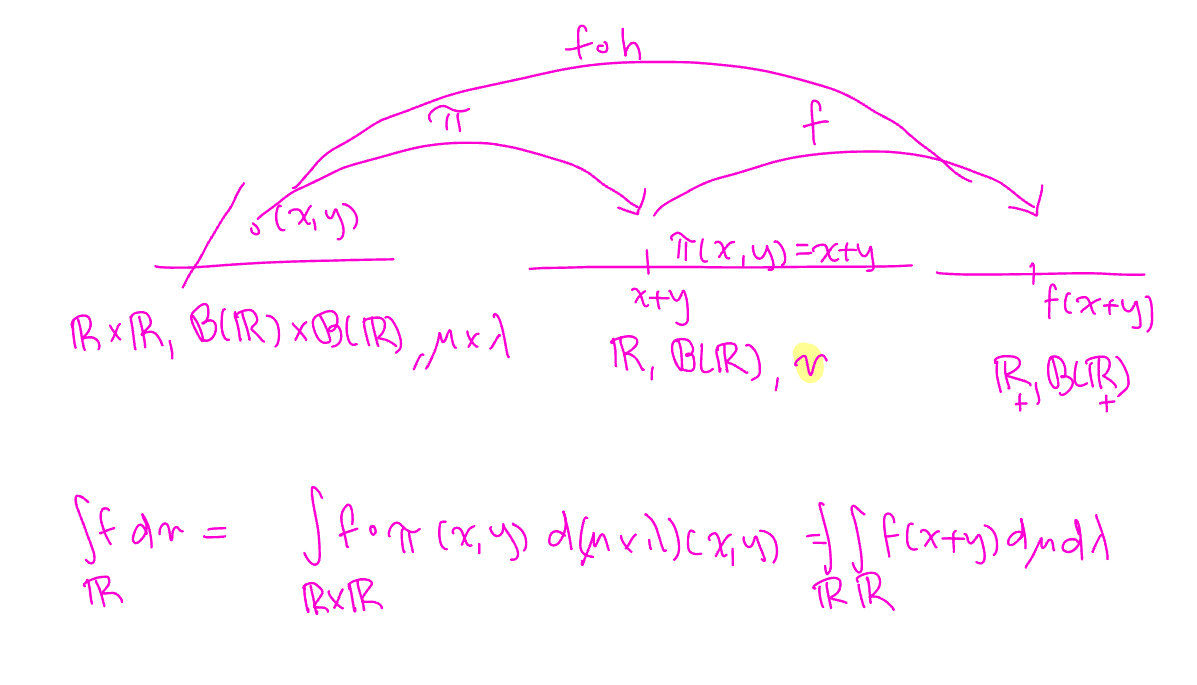
\includegraphics[width=0.75\linewidth]{hw10q1a.png}
                \caption{Work for Problem 1, Part A}
            \end{figure}
            
        \end{proof}
        
        \item[(b)] Show that 
        \[\nu(A) = \int_{\real} \mu(A - t)\lambda(dt), \: A \in \borel\]

        \begin{proof}
            Let $A \in \borel$ be given \\
            $\nu(A) \equiv (\mu * \lambda)(A) \equiv \int_\real \int_\real I_A(x + t) d \mu(x) d\lambda(t)$ \\
           (We can hold t constant) \\
            = $\int_\real\int_\real I_{A-t}(x) d \mu(x) d\lambda(t)$ \\
            = $\int_\real \mu(A-t) d\lambda(t)$
        \end{proof}
        
        \item[(c)] Suppose there exist countable sets $B_\lambda$ and $B_\mu$ such that $\mu(B_\mu^c) = 0 = \lambda(B_\lambda^c)$. Show that there exists a countable set $B_\nu$ such that $\nu(B^c_\nu) = 0$ 

        \begin{proof}
            $B_\nu \equiv B_\lambda + B_\mu = \{x + y | x \in B_\mu, y \in B_\lambda\}$

            Keeping in mind: $\mu(B_\mu^c) = \int I_{B_\mu^c}(x) d \mu(x)$ and $\lambda(B_\lambda^c) = \int I_{B_\lambda^c}(y) d \lambda(y)$

            $I_{B_\mu^c + B_\lambda^c}(x+y) \leq I_{B_\mu^c}(x) + I_{B_\lambda^c}(y)$ because:
            \begin{itemize}
            \item $I_{B_\mu^c + B_\lambda^c}(x+y) = 1 \implies x \in B_\mu, y \in B_\lambda \implies I_{B_\mu^c}(x) + I_{B_\lambda^c}(y) = 2 \implies I_{B_\mu^c + B_\lambda^c}(x+y) < I_{B_\mu^c}(x) + I_{B_\lambda^c}(y)$
            \item $I_{B_\mu^c + B_\lambda^c}(x+y) = 0 \implies$ either
            \begin{itemize}
                \item $x \in B_\mu, y \notin B_\lambda \implies I_{B_\mu^c}(x) + I_{B_\lambda^c}(y) = 1 \implies I_{B_\mu^c + B_\lambda^c}(x+y) < I_{B_\mu^c}(x) + I_{B_\lambda^c}(y)$
                \item $x \notin B_\mu, y \in B_\lambda \implies I_{B_\mu^c}(x) + I_{B_\lambda^c}(y) = 1 \implies I_{B_\mu^c + B_\lambda^c}(x+y) < I_{B_\mu^c}(x) + I_{B_\lambda^c}(y)$
                \item $x \notin B_\mu, y \notin B_\lambda \implies I_{B_\mu^c}(x) + I_{B_\lambda^c}(y) = 0 \implies I_{B_\mu^c + B_\lambda^c}(x+y) = I_{B_\mu^c}(x) + I_{B_\lambda^c}(y)$
            \end{itemize}
            \end{itemize}
            $\nu(B_\lambda^c) = \int\int I_{B_\nu^c}(x+y)d\mu(x) d \lambda(y) \leq \int I_{B_\mu^c}(x)d\mu(x) + \int I_{B_\lambda^c}(y)d \lambda(y) = 0$
        \end{proof}
        \item[(d)] Suppose that $\mu(\{x\})= 0$ for all x in $\real$. Show that $\nu(\{x\}) = 0$ for all x in $\real$ 
        \begin{proof}
        Let $x \in \real$ be given.
            \begin{align*}
                & \nu(\{x\}) = \int_\real \mu(\{x\} - y) \lambda(dy) && (\textrm{from part (b)}) \\
                & = \int_\real \mu(\{x - y\}) \lambda(dy) \\
                & = \int_\real 0 \lambda(dy) && ((\textrm{since } x - y \in \real) \\
                 & =0
            \end{align*}
        \end{proof}
        \item[(e)] Suppose that $\mu << m$ with $\frac{d \mu}{dm} = h$. Show that $\nu << m$ and find $\frac{d\nu}{dm}$ in terms of $h$, $\mu$, and $\lambda$.
        \item[(f)] Suppose that $\mu << m$ and $\lambda << m$. Show that:
        \[\frac{d \nu}{dm} = \frac{d\mu}{dm}*\frac{d \lambda}{dm}\]
    \end{itemize}
    

    
\clearpage
%%%%%%%%%%% Question 2 %%%%%%%%%%%%%%%%%%%%    
    \question \textbf{Chapter 5 Problem 14}: (Hint: use the continuous version of DCT, i.e problem 2.22)

    Let $f, g \in L^1(\real, \borel, m)$.
    \begin{itemize}
        \item[(a)] Show that if $f$ is continuous and bounded on $\real$, then so is $f * g$.
        \item[(b)] Show that if $f$ is differentiable with a bounded derivative on $\real$, then so if $f * g$ 
    \end{itemize}
    \begin{solution}
        
    \end{solution}
\clearpage
%%%%%%%%%%% Question 3 %%%%%%%%%%%%%%%%%%%%    
    \question \textbf{Chapter 5 Problem 15(a)}: (skip the equality part at the end!)

    Let $f \in L^1(\real)$, $g \in L^p(\real)$, $ 1 \leq p \leq \infty$

    Show that if $1 \leq p < \infty$, then for all $x \in \real$
    \[\left|\int|f(u)-g(x-u)|du\right|^p \leq \left(\int|f|dm\right)^{p-1} \left(\int|g(x - u)|^p|f(u)|du\right)\]
    and hence that 
    \[(f*g)(x) \equiv \int f(u)g(x - u)du\]
    is well defined a.e.(m)
    \begin{solution}
        
    \end{solution}
\clearpage
%%%%%%%%%%% Question 4 %%%%%%%%%%%%%%%%%%%%    
    \question \textbf{Problem A}

    Problem A: Let $\mu$, $\lambda$ be two probabilities on $(\real, \borel)$. Consider the functions $f (x, y) = x$, $g(x, y) = y$ defined from $(\real^2, \calB(\real^2)$, $\nu \equiv \mu \times \lambda)$ to $(\real, \borel)$. It is easy to see that these are measurable transformations, i.e random variables (Prove it if you don’t see it!). Assume $f, g \in L^2(\real^2, B(\real^2), \nu)$. Then show the following two facts:
    \[\nu(\{f \in A\} \cap \{g \in B\}) \equiv \nu(\{(f, g) \in A \times B\}) = \nu(\{f \in A\}) \nu(\{g \in B\}), \: \forall \: A, B \in \borel\]
    \[\int fg d\nu = \left(\int f d \nu\right) \left(\int g d\nu\right)\]
    \textit{[Recall our notation} $\{f \in A\} \equiv \{(x, y) : f (x, y) \in A\} \equiv f^{-1}(A)$.
    \textit{Hint: May have to use Cauchy Schwarz first!]}
    
    \textbf{Measure theory Trivia:} Can you interpret this fact in terms of independent random variables?

    \begin{solution}
    \begin{proof}
    Let $A, B \in \borel$ be given.
    \begin{align*}
        & \nu(\{f \in A\} \cap \{g \in B\}) \\
        & = \nu(\{(x, y) \in \real^2: x \in A, y \in \real\}\cap \{(x, y) \in \real^2: x \in \real, y \in B\}) \\
        & = \nu(\{(x, y) \in \real^2: x\in A, y\in B\}) \\
        & = \nu(\{(f, g) \in A\times B\})
    \end{align*}

    By Theorem 5.1.2, we know that $\nu_1(A \times B) = \nu_2(A \times B) = \nu(A \times B)$

    Thus, by (iii), $\nu(\{(f, g) \in A\times B\}) = \nu(\{f \in A\})\nu(\{g \in B\}) $

    
    \end{proof}
    \textbf{Trivia Answer:} If we have 2 independent random variables $X, Y$ on a probability space $(\Omega, \calF, P)$, 
    $P(X\in A, Y \in B) = P(X \in A) P(Y \in B)$ and $E(XY) = EXEY$
    \end{solution}
\clearpage
%%%%%%%%%%% Question 5 %%%%%%%%%%%%%%%%%%%%    
    \question \textbf{Problem B}

    B. Let $f = \one_A$, $g = \one_B$ be two indicator functions for sets $A, B \in \borel$. Express the convolution function $(f * g)(x)$ in terms of lebesgue measure of sets, for each $x \in \real$.
    \begin{solution}
        Let $x \in \real$ be given. 
        
        From definition 5.4.4: 
        \begin{align*}
            & f*g(x) = \int f(x - u) g(u) du \\
            & = \int \one_A(x - u) \one_B(u) du \\
            & = \int \one_{x - A}(u) \one_{B}(u) du && (x\textrm{ is fixed}) \\
            & = \int \one_{x - A \cap B}(u)du \\
            & = \int \one_{x - A \cap B} dm \\
            & = m(x - A \cap B)
        \end{align*}
    \end{solution}
\clearpage
%%%%%%%%%%% Question 6 %%%%%%%%%%%%%%%%%%%%    
    \question \textbf{Chapter 6 Problem 1}

    Let $\mu_1 = \mu_2$ be the probability distribution on $\Omega = \{1, 2\}$ with $\mu_1(\{1\}) = 1/2$. Find 2 distinct probability distributions on $\Omega \times \Omega$ with $\mu_1$ and $\mu_2$ as the set of marginals. 
    \begin{solution}
    1) The product measure: $\mu_1 \times \mu_2$        FIX ME
    \end{solution}
\clearpage
%%%%%%%%%%% Question 7 %%%%%%%%%%%%%%%%%%%%    
    \question \textbf{Chapter 6 Problem 3}

    In the change of variables formula, one of the three integrals is usually easier to evaluate than the other two. In this problem, in part (a), the first integral is easier to evaluate than the other two while in part (b), the second one is easier.
    \begin{itemize}
        \item[(a)] Let $Z \sim N(0, 1), \: X = Z^2$, and $Y = e^{-X}$
        \begin{itemize}
            \item[(i)] Find the distributions $P_X$ and $P_Y$ on $(\real, \borel)$
            \item[(ii)] Compute the integrals
            \[\int_{\real} e^{-z^2}\phi(z)dz, \: \int_{\real}e^{-x}P_X(dx), \: \& \: \int_{\real} y P_Y(dy)\]
            where $\phi(z) = \frac{1}{\sqrt{2\pi}}e^{-z^2/2}, \: -\infty < z < \infty$. Verify that all 3 integrals agree.
        \end{itemize}
        \item[(b)] Let $X_1, X_2, ... , X_n$ be iid N(0, 1) random variables. Let $Y = (X_1 + X_2 + ... + X_k)$ and $Z = Y^2$
        \begin{itemize}
            \item[(i)] Find the distributions of $Y$ and $Z$ 
            \item[(ii)] Evaluate $\int_{\real^k}(x_1 + ... x_k)^2 dP_{X_1, X_2, ... , X_k}(x_1, ... , x_k),$ $\int_{\real}y^2P_Y(dy)$, and $\int_{\real_+}zP_Z(dz)$ 
        \end{itemize}
        \item[(c)] Let $X_1, X_2, ... , X_n$ be Binomial $(n_i, p)$, $i = 1, 2, ..., k$ random variables. Let $Y = (X_1 + X_2 + ... + X_k)$
        \begin{itemize}
            \item[(i)] Find the distributions of $Y$ and $Z$ 
            \item[(ii)] Evaluate $\int_{\real^k}(x_1 + ... x_k) dP_{X_1, X_2, ... , X_k}(x_1, ... , x_k)$ and $\int_{\real}yP_Y(dy)$ 
        \end{itemize}
    \end{itemize}

    \begin{solution}
        (a) \\
        (i) \\
        \underline{CDF of X}: 
        \begin{align*}
            & P_X((-\infty, x]) = P(\{\omega: X(\omega) \leq x\}) \\
            & = P(\{\omega: (Z(\omega))^2 \leq x \}) = P(\{\omega: -\sqrt{x} \leq Z(\omega) \leq \sqrt{x} \}) \\
            & = \one_{\{x \geq 0\}}(\Phi(\sqrt{x}) - \Phi(-\sqrt{x})) = 2\one_{\{x \geq 0\}}\Phi(\sqrt{x})
        \end{align*}
        \underline{CDF of Y}: 
        \begin{align*}
            & P_Y((-\infty, y]) = P(\{\omega: Y(\omega) \leq y\}) \\
            & = P(\{\omega: e^{-Z(\omega)} \leq x \}) = P(\{\omega:  Z(\omega) \geq -\log(y) \}\one_{\{y > 0\}}) \\
            & = \one_{\{y \geq 1\}}(1 - \Phi(-\log(y))) \\
        \end{align*}
        (ii) \begin{align*}
            & \int_{\real} e^{-z^2}\phi(z)dz = \int_{\real} e^{-z^2}\frac{1}{\sqrt{2\pi}}e^{-z^2/2}dz \\
            & = \int_{\real} \frac{1}{\sqrt{2\pi}}e^{-3z^2/2}dz = \sqrt{\frac{1}{3}}\int_{\real} \frac{1}{\sqrt{\frac{2}{3}\pi}}e^{-z^2/(\tfrac{2}{3})}dz = \sqrt{\frac{1}{3}} \times 1 = \sqrt{\frac{1}{3}}
        \end{align*}
    \end{solution}
\clearpage
%%%%%%%%%%% Question 8 %%%%%%%%%%%%%%%%%%%%    
    \question \textbf{Chapter 6 Problem 6}

    Show that if equality holds in (2.20), then there exist constants $a$ and $b$ such that $P (Y = aX + b)=1$. (Hint: Show that there exist a constant $a$ such that $Var(Y - aX)= 0$.)

    \textbf{Proposition 6.2.8:} Cauchy Schwarz inequality) which contains (2.20). Let $X$ and $Y$ be random variables on $(\Omega, \calF, P)$ with $E|X|^2 < \infty$ and $E|Y|^2 < \infty$. Then:
    \[|Cov(X, Y)| \leq \sqrt{Var(X)}\sqrt{Var(Y)}\]
    Where $Cov(X, Y) = EXY - EXEY$.

    \begin{solution}
        
    \end{solution}


\end{questions}
\end{document}